
This section  describes the $\pi$-SOD-M development environment that implements the generation of {\em A-policies}' based services' compositions. For a given services' based application, the process  consists in generating the  code starting from a $\pi$-SCM modeling an application. Note that the services' composition model is not modeled from scratch, but it is the result of a general process defined by the $\pi$-SOD-M method in which a set of models are built following a service oriented approach \cite{decastro1}.

%We used the Eclipse Modeling Framework (EMF) to implement the whole model transformation process \footnote {The EMF project is a modeling framework and code generation facility for building tools and other applications based on a structured data model.}. From a model specification described in XMI, EMF provides tools and runtime support to produce a set of Java classes for the model, along with a set of adapter classes that enable viewing and command-based editing of the model, and a basic editor.
%In order to automate the transformation we specified  transformation rules using the ATL model transformation language Finally, in order to generate code we  used Acceleo \footnote{http://www.acceleo.org/pages/home/en}.

%%..--..--..--..--..--..--..--..--..--..--..--..--..--..--..--..--..--..--..--..--..--..--..--..--..--..--..--..--..--..--..--..--..--..--..--..--..--..--
\subsection{General architecture}
%%..--..--..--..--..--..--..--..--..--..--..--..--..--..--..--..--..--..--..--..--..--..--..--..--..--..--..--..--..--..--..--..--..--..--..--..--..--..--

Figure \ref{fig:policymanager} depicts a general architecture of the $\pi$-SOD-M Development Environment showing the set of plug-ins  developed in order to implement it. The environment implements the abstract architecture. Thus, it consists of plug-ins implementing the $\pi$-SCM and $\pi$-{\sc Pews} meta-models used for defining models specifying services' compositions and their associated policies; and ATL rules for transforming  PSM models (model to model transformation) and finally generating code (model to text transformation).
\begin{figure}[t]
	\begin{center}
		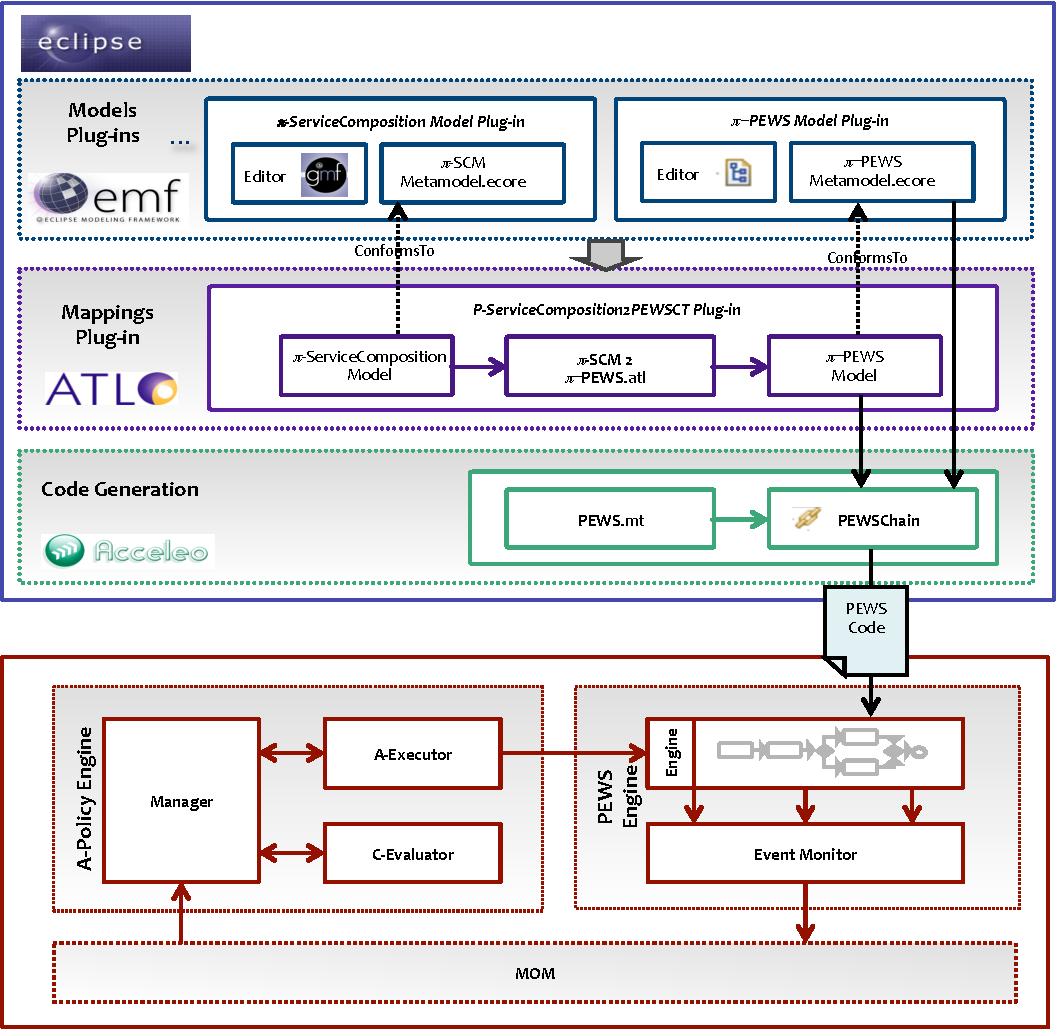
\includegraphics[width=0.60\textwidth]{figs/architecture}
	\end{center}
		\caption{$\pi$-SOD-M Development Environment}
   \label{fig:policymanager}
\end{figure}
\begin{itemize}
\item 	We  used the Eclipse Modeling Framework (EMF) \footnote {The EMF project is a modeling framework and code generation facility for building tools and other applications based on a structured data model.}   for implementing the meta-models  $\pi$- SCM and $\pi$-{\sc Pews}. Then, starting form these meta-models, we  developed the models' plug-ins needed to support the graphical representation of the $\pi$- SCM and $\pi$-{\sc Pews} models ($\pi$-ServiceCompostion Model and $\pi$-PEWS Model plug-ins).

\item	 We used  ATL \footnote{http://eclipse.org/atl/. An ATL program is basically a set of rules that define how source model elements are matched and navigated to create and initialize the elements of the target models.}
for  developing the mapping plug-in implementing the  mappings between models ($\pi$-ServiceComposition2$\pi$-PEWS Plug-in).

\item 	We  used Acceleo \footnote{http://www.acceleo.org/pages/home/en} for implementing  the code generation plug-in. We coded the pews.mt program  that implements the model to text transformation for generating executable code. It takes as input a $\pi$-PEWS model implementing a specific services' composition and it generates the code to be executed by the 
{\em A-policy} based services' composition execution environment. 

%\item Finally, we created a chain execution  to execute the model to text transformation.
\end{itemize}

%..--..--..--..--..--..--..--..--..--..--..--..--..--..--..--..--..--..--..--..--..--..--..--..--..--..--..--..--..--..--..--..--..--..--..--..--..--..--
\subsection{Transformation rules}\label{sec:mmrules}
%..--..--..--..--..--..--..--..--..--..--..--..--..--..--..--..--..--..--..--..--..--..--..--..--..--..--..--..--..--..--..--..--..--..--..--..--..--..--

Figure \ref{fig:transformations} shows the transformation principle between the elements of the $\pi$-SCM meta-model used for representing the services' composition into the elements of the $\pi$-{\sc Pews} meta-model. There are two groups of rules: those that transform services' composition elements of the $\pi$-SCM to $\pi$-{\sc Pews} meta-models elements; and those that transform rules grouped by policies into {\em A-policy} types.

% _ . _ . _ . _ . _ . _ . _ . _ . _ . _ . _ . _ . _ . _ . _ . _ . _ . _ .
%\noindent

%{\bf\em 
\subsubsection{Transformation of the services' composition elements of the $\pi$-SCM to the $\pi$-{\sc Pews} elements}
% _ . _ . _ . _ . _ . _ . _ . _ . _ . _ . _ . _ . _ . _ . _ . _ . _ . _ .
A named action of the $\pi$-SCM represented by  {\sc\em Action} and {\sc\em Action:name} is transformed to a  named class {\sc Operation} with a corresponding attribute name {\sc Operation:name}. A  named service activity represented by the elements {\sc\em ServiceActivity}  and  {\sc\em ServiceActivity:name} of the $\pi$-SCM, are  transformed into a named operation of the $\pi$-{\sc Pews} represented by the elements  {\sc CompositeOperation} and {\sc CompositeOperation:name}. When more than one action is called, according to the following  composition patterns expressed using the operators {\sc\em merge, decision, fork and join} in the $\pi$-SCM the corresponding transformations, according to the PEWS operators presented above, are (see details in Figure \ref{fig:transformations}):
\begin{itemize}
\item   $op_1 . op_2$ if no {\sc\em ControlNode} is specified
\item ($op_1 \parallel op_2) . op_3$ if control nodes of type {\sc\em fork, join} are combined
 \item ($op_1 + op_2) . op_3$ if control nodes of type {\sc\em decision, merge} are combined
\end{itemize}

In the scenario "To Publish Music" the service activity {\sf PublishMusic} of the $\pi$-SC model specifies  calls to two {\sf Activitie}s of type {\em UpdateMusic}, respectively concerning the {\sf Business Service}s {\em Facebook} and {\em Twitter}. Given that no {\sf ConstrolNode} is specified by the $\pi$-SC model, the corresponding transformation is the expression that defines a {\sf Composite Operation} named {\em PublishSong} of the $\pi$-{\sc Pews} model of the form ({\sf PublishFacebook} $\parallel$ {\sf PublishTwitter}).
\begin{figure}
\centering{
%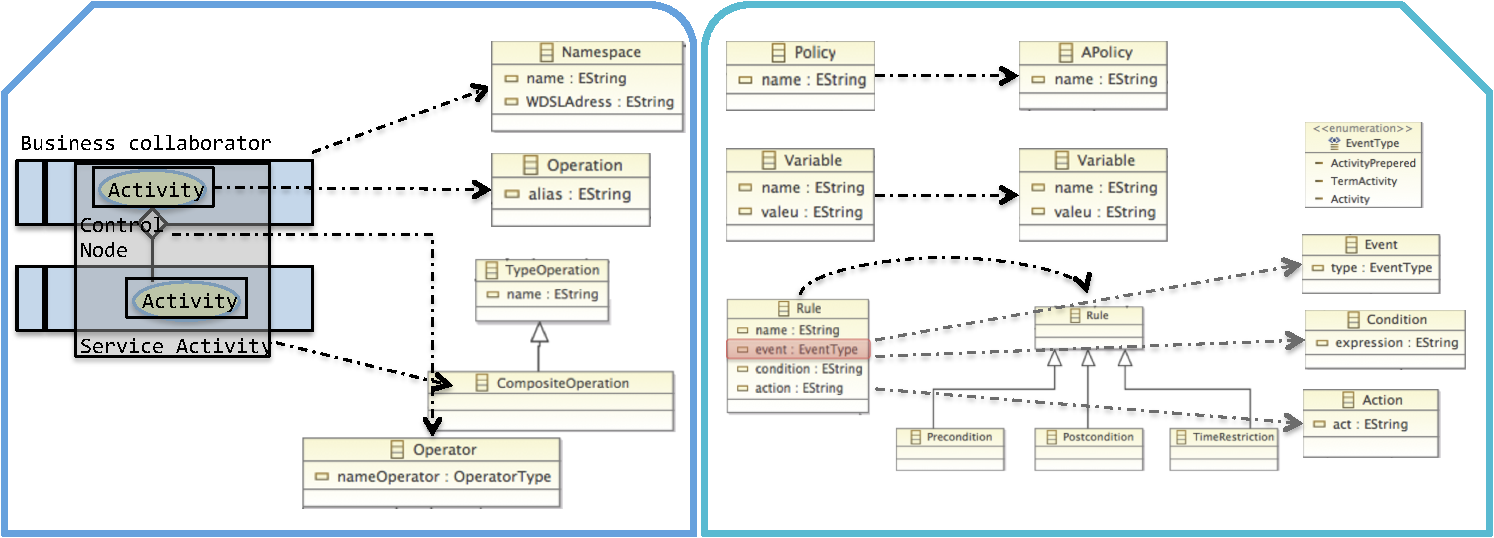
\includegraphics[width=0.80\textwidth]{figs/PI-SC-PI-P}}
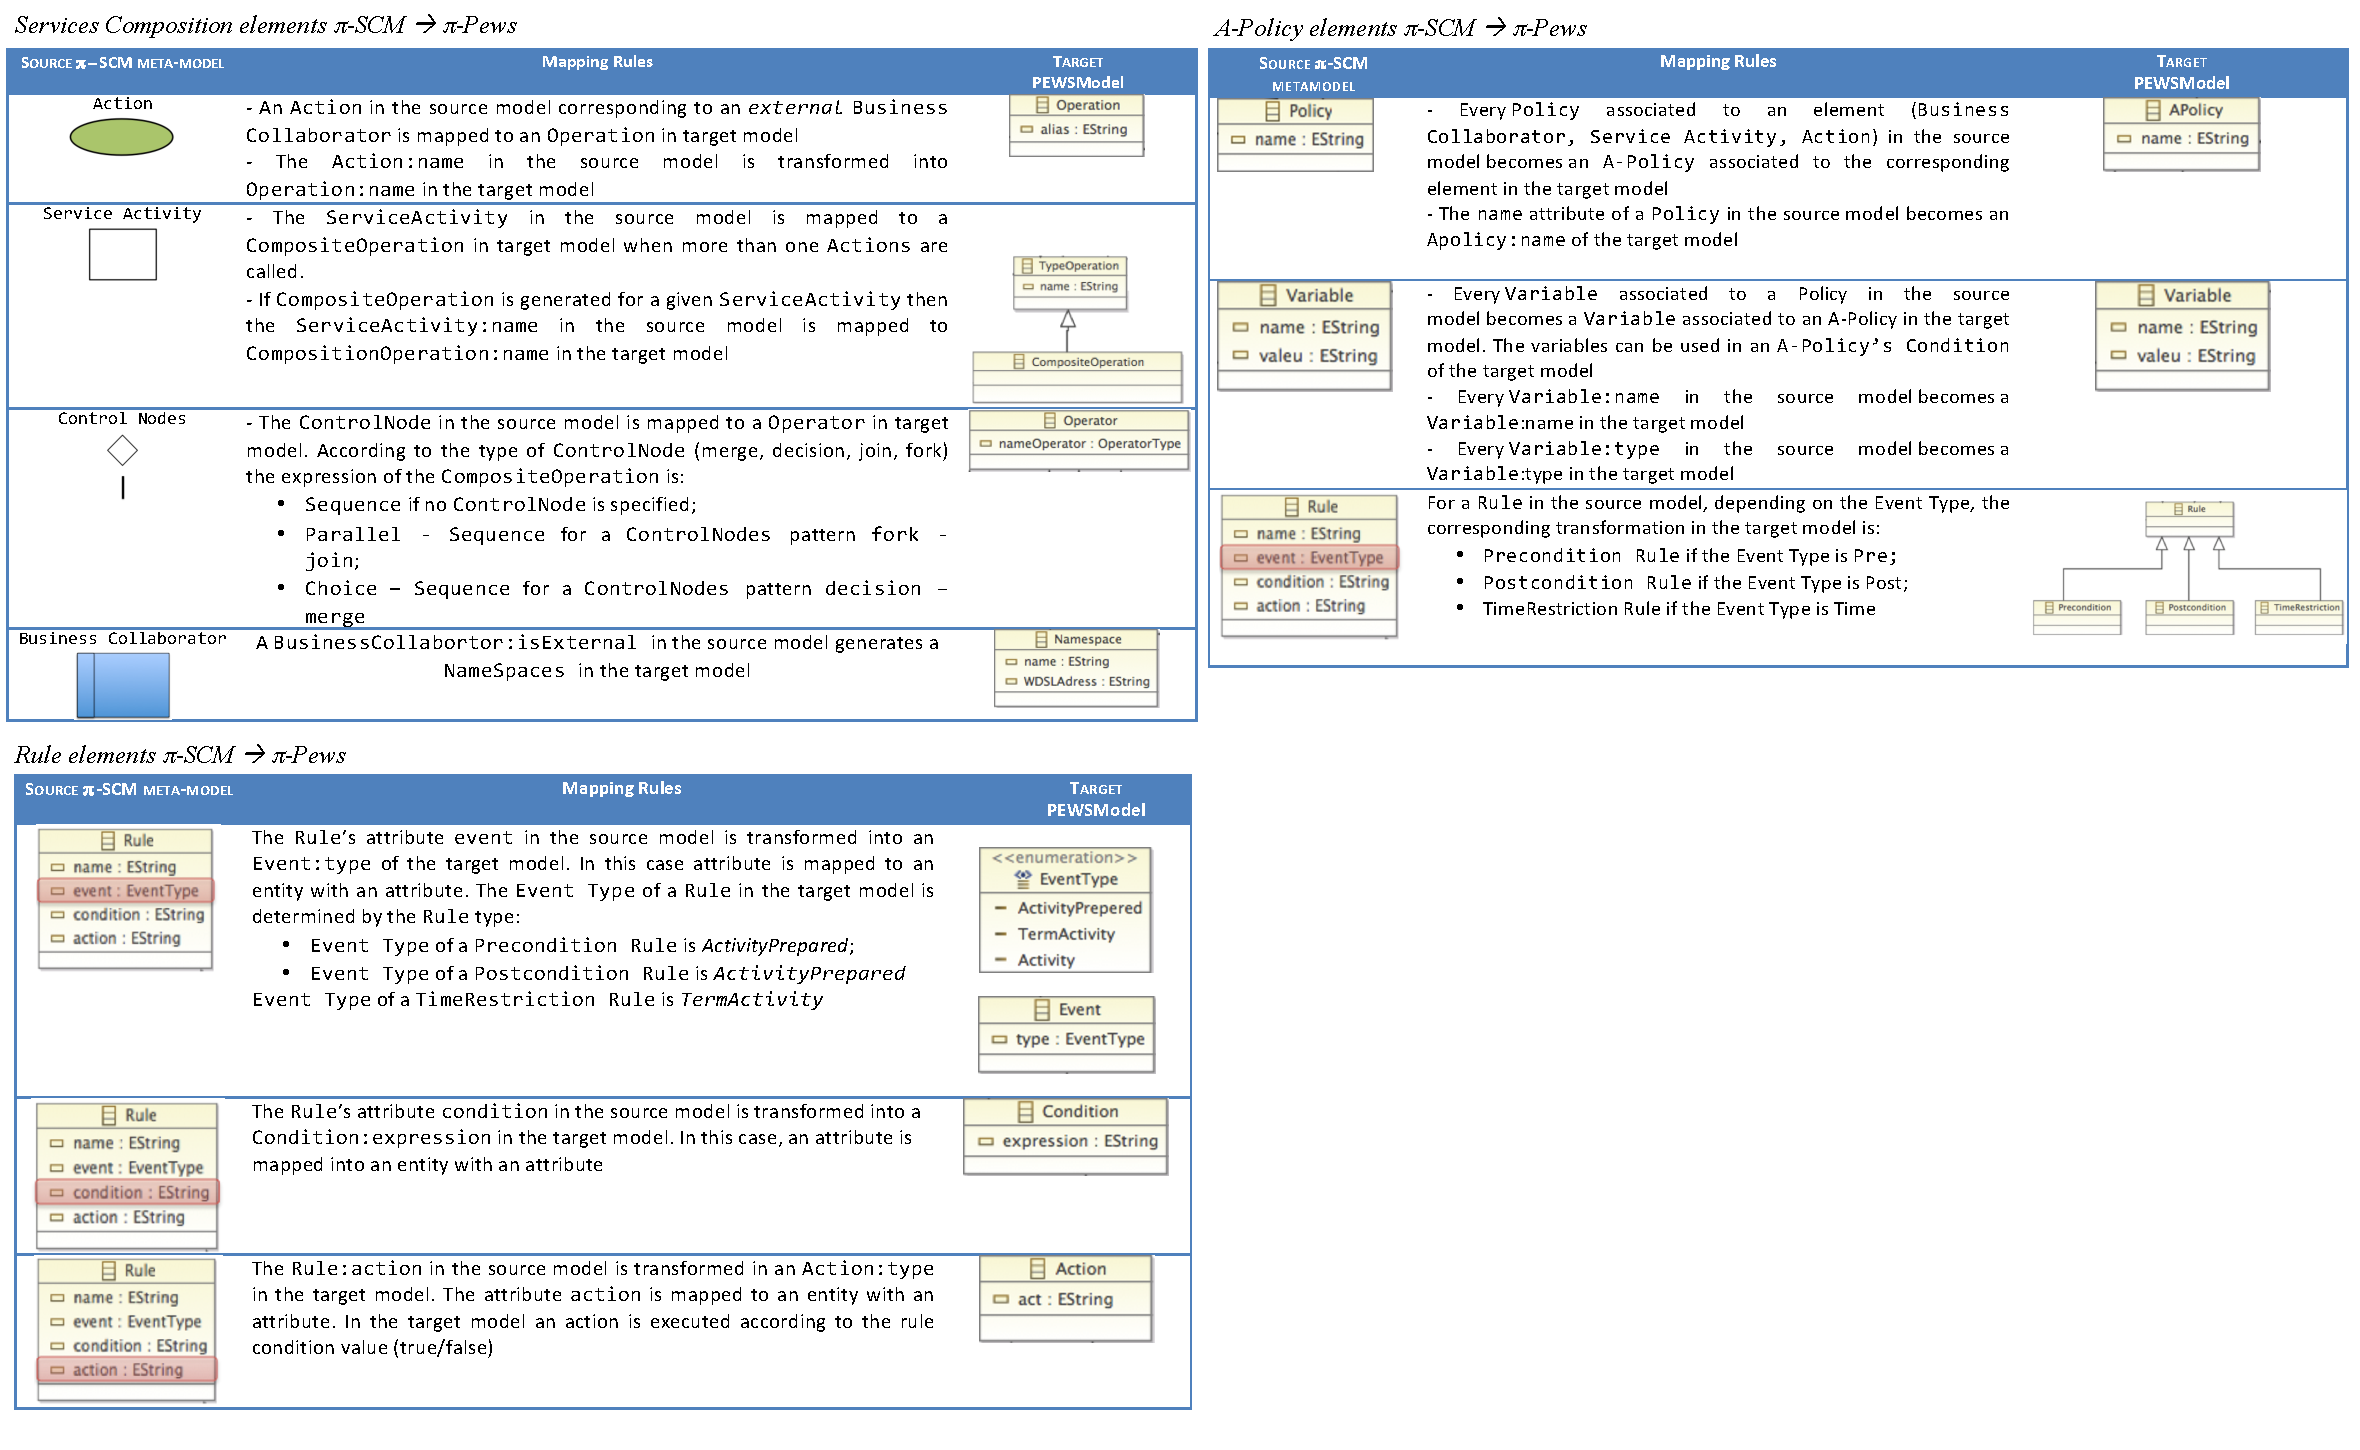
\includegraphics[width=0.96\textwidth]{figs/Mapping-1}}
\caption{ $\pi$-SCM to $\pi$-{\sc Pews} transformation}
\label{fig:transformations}
\end{figure}

% _ . _ . _ . _ . _ . _ . _ . _ . _ . _ . _ . _ . _ . _ . _ . _ . _ . _ .
%\noindent

%{\bf\em 
\subsubsection{Transformation of rules grouped by A-policies   in the $\pi$-SCM to A-Policies of  $\pi$-{\sc Pews}}
% _ . _ . _ . _ . _ . _ . _ . _ . _ . _ . _ . _ . _ . _ . _ . _ . _ . _ .
The {\em A-policies} defined for the elements of the $\pi$-SCM are transformed into {\sc A-Policy} classes, named according to the names expressed in the source model. The transformation of the rules expressed in the $\pi$-SCM is guided by the event types associated to these rules.   The variables associated to an {\em A-policy} expressed in the $\pi$-SCM as {\sc\em $<$Variable:name, Variable:type$>$} are transformed into elements of type {\sc Variable} with attributes {\sc name} and {\sc type} directly specified from the elements {\sc\em  Variable:name} and {\sc\em Variable:type} of the $\pi$-SCM model.

As shown in Figure \ref{fig:transformations}, for an event of type {\sc\em Pre} the corresponding transformed rule is of type {\sc Precondition}; for an event of type {\sc\em Post} the corresponding transformed rule is of type {\sc Postcondition}; finally, for an event of type {\sc\em TimeRestriction} the corresponding transformed rule is of type {\sc Time}. 
The condition expression of a rule in the $\pi$-SCM ({\sc\em Rule:condition}) is transformed into a class {\sc\em Condition:expression} where the attributes of the expression are transformed into elements of type {\sc Attribute}.

%The attribute event of a rule  ({\sc\em Rule:event}) in the $\pi$-SCM is transformed into an {\sc Event Type} according to the rule type. 

%As shown in Figure \ref{fig:transformations}, the event type for a rule of type (i) {\sc Precondition} is {\sc ActivityPrepared}; (ii) {\sc Postcondition} is {\sc TermActivity}; (iii) {\sc TimeRestriction} is {\sc Temporal}. The {\sc\em Rule:Action} of a rule in the $\pi$-SCM is transformed into an {\sc Action:type}.

%
%Figure \ref{fig:p-scim} shows the  $\pi$-{\sc Pews} model for our example.
In the scenario "To Publish Music" the {\sf Policies} {\em OAuthPolicy} and {\em HTTPAuthPolicy} of the $\pi$-SCM model are transformed into {\em A-policies} of type {\sf Precondition} of the $\pi$-{\sc Pews} model of the scenario. Thus in both cases the events are of type {\sf ActivityPrepared}. These policies, as stated in the $\pi$-SCM model, are associated to {\sf Activities}. In the corresponding transformation they are associated to {\sf Operation}s {\em PublishFacebook} and {\em PublishTwitter}.
%\begin{figure}[htpb]
%\centering{
%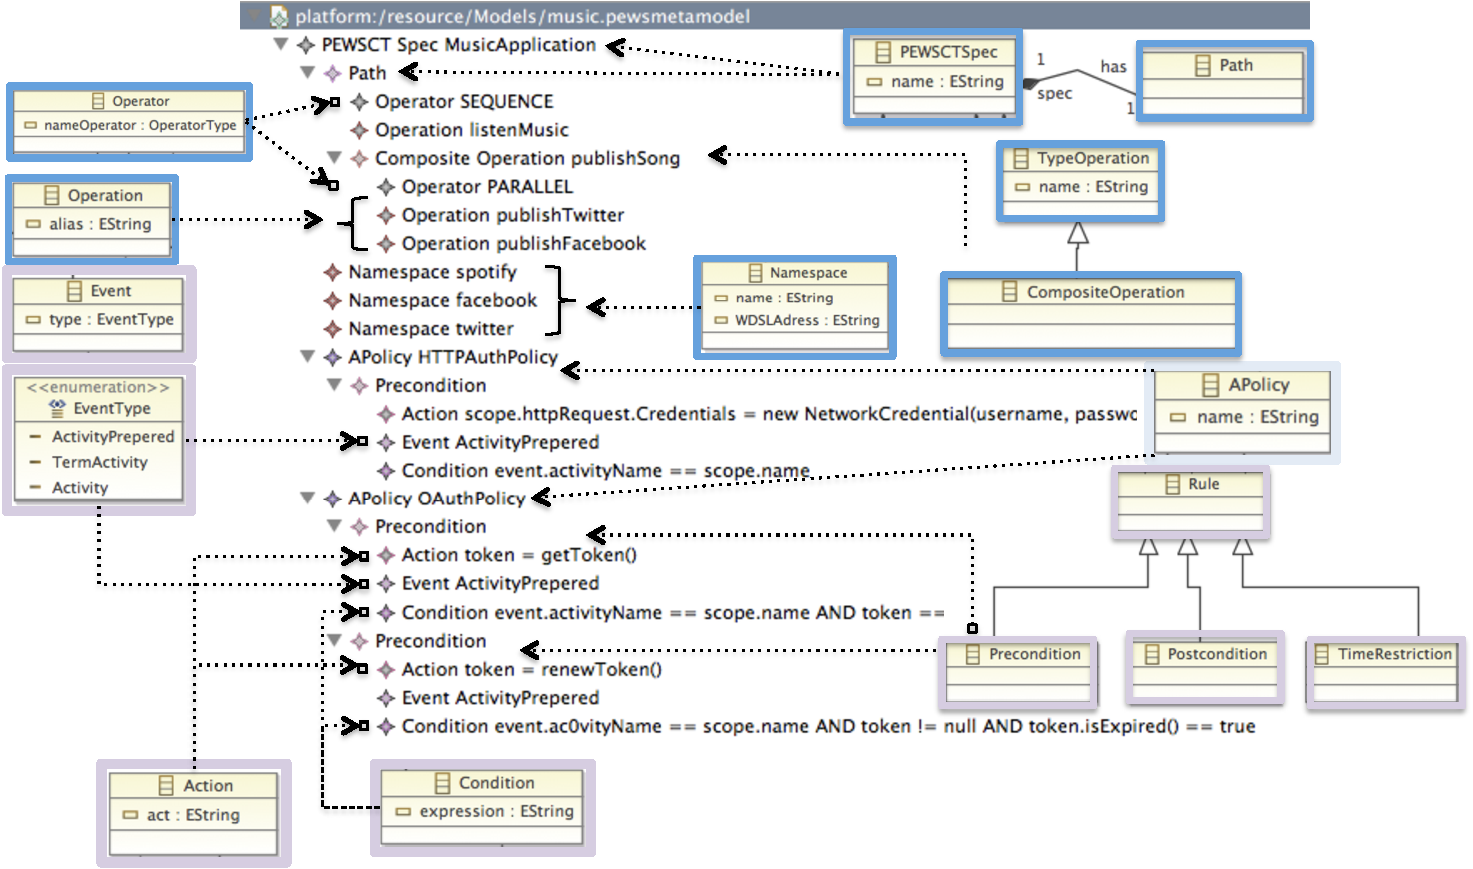
\includegraphics[width=0.78\textwidth]{figs/modeloPEWS}}
%\caption{$\pi$-{\sc Pews} generated model fo the "To Publish Music" application}
%\label{fig:p-scim}
%\end{figure}

%Figure \ref{fig:pewsexpression} shows the correspondence between the model and the statements that implement it, with a schematic representation of the business process.
%\begin{figure}
%\centering{
%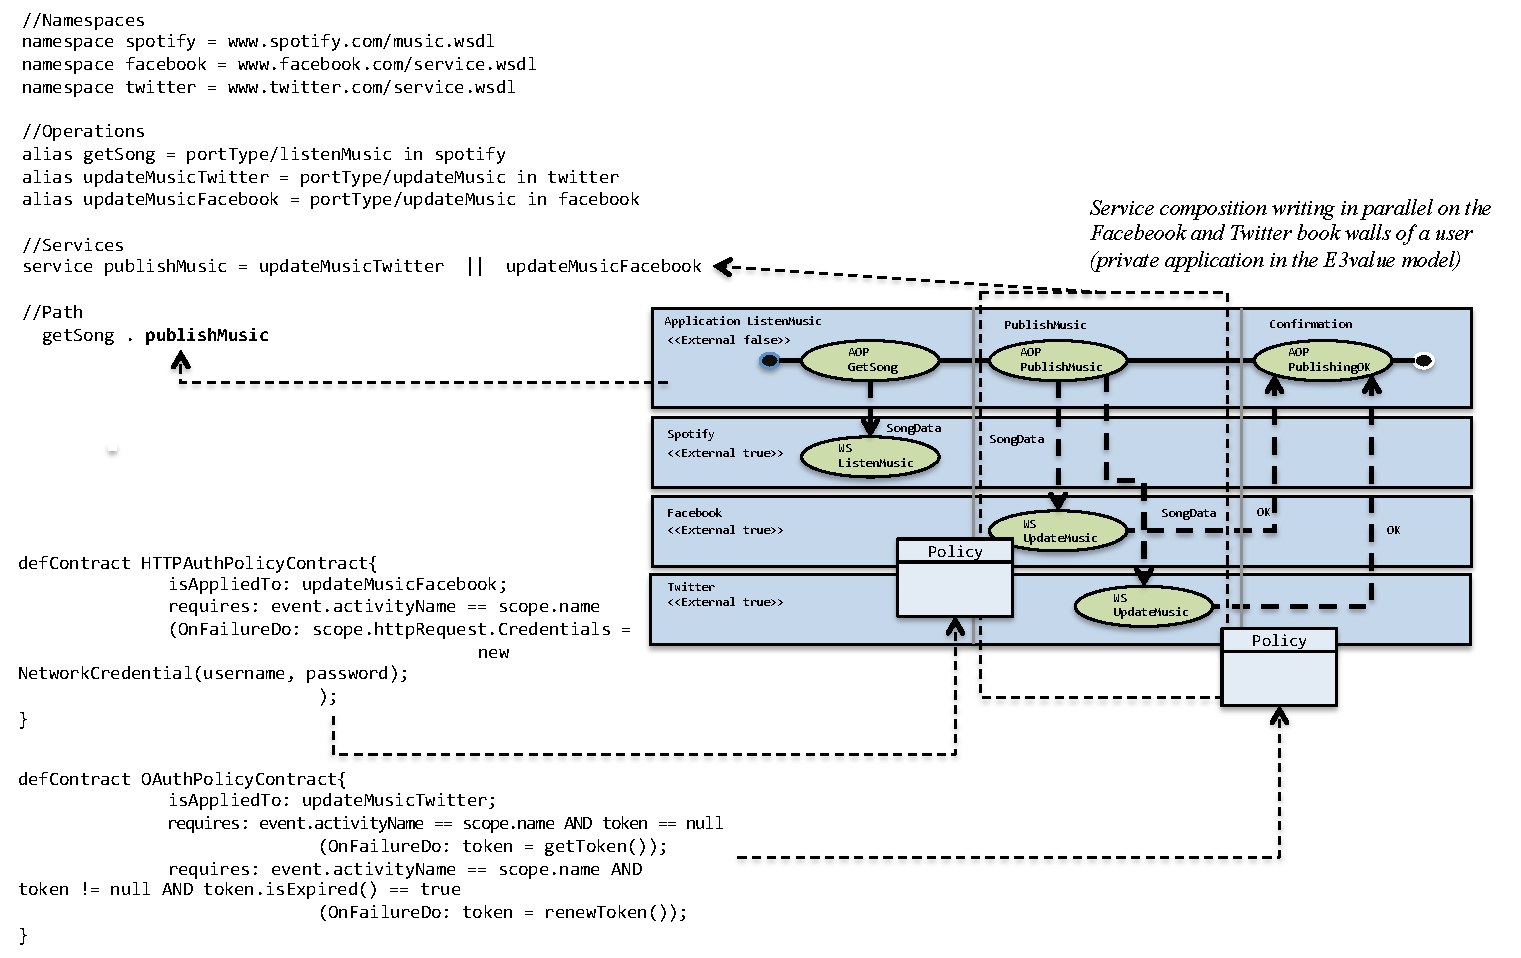
\includegraphics[width=0.85\textwidth]{figs/pews-expression}}
%\caption{Pews program implementing the "To Publish Music" application}
%\label{fig:pewsexpression}
%\end{figure}

%%..--..--..--..--..--..--..--..--..--..--..--..--..--..--..--..--..--..--..--..--..--..--..--..--..--..--..--..--..--..--..--..--..--..--..--..--..--..--
\subsection{A-policy manager}
%..--..--..--..--..--..--..--..--..--..--..--..--..--..--..--..--..--..--..--..--..--..--..--..--..--..--..--..--..--..--..--..--..--..--..--..--..--..--

As  shown in Figure \ref{fig:policymanager}, once an instance of a PEWS code is obtained starting form a particular $\pi$-services' composition model it can be executed over {\em A-policy} based services' composition execution environment  consisting of a composition engine and a {\em A-policy} manager.  The  {\em A-policy} manager  consists of three main components Manager, for scheduling the execution of rules, C-Evaluator and A-Executor respectively for evaluating rules' conditions and executing their actions. The {\em A-policy} Manager interacts with a composition engine thanks to a  message communication layer (MOM).


The composition engine manages the life cycle of the composition. Once a composition instance is activated, the engine schedules the composition activities according to the composition control flow.
Each activity is seen as the process where the service method call is executed.
The execution of an activity has four states: prepared, started, terminated, and failure.
The execution of the control flow (sequence, and/or split and join) can also be prepared, started, terminated and raise a failure.

At execution time, the evaluation of policies done by the {\em A-policy} manager must be synchronized with the execution of the services' composition (i.e., the execution of an activity or a control flow).  Policies associated to a scope are activated when the execution of its scope starts. A {\em A-policy} will have to be executed only if one or several of its rules is triggered. If several rules are triggered the {\em A-policy} manager first builds an execution plan that specifies the order in which such rules will be executed according to the strategies defined in the following section. 
%Once rules have been executed, the {\em A-policy} finishes its execution and returns to a sleeping state.
If rules belonging to several policies are triggered then policies are also ordered according to an execution plan. The execution of policies is out of the scope of this paper, the interested reader can refer to \cite{Espinosa-Oviedo2011a} for further details.
%The order of policies has implications on the global order of the rules to be executed.



